The reconstruction of ancestral languages depends on structural regularities that persist across phonological evolution. Sound change occurs according to consistent patterns that affect entire grammatical systems. These patterns allow historical inference to proceed by rule-governed comparison rather than conjecture. When multiple daughter languages show aligned differences in equivalent words, the shape of the ancestral form can often be inferred with precision.

Historical linguistics treats shared morphological and syntactic structures as stronger indicators of genealogical descent than surface-level lexical similarity. Formal correspondences in case endings, agreement systems, and word order provide durable signals of common ancestry. These structural features must appear across a wide range of lexical items to count as evidence for descent. Chance resemblance or cultural borrowing cannot produce such system-wide alignment.

Proto-Indo-European (PIE) is the name assigned to the unattested language reconstructed from structural parallels among Indo-European languages. Its existence is inferred from regularities in grammar and phonology shared by Sanskrit, Ancient Greek, Latin, Hittite, Old Church Slavonic, and others. These languages exhibit consistent transformations that imply a common origin. The reconstructed forms of PIE reflect the points of maximal convergence across its descendants.

The comparative method identifies systematic sound correspondences that link descendant languages to a shared root. For example, Latin \emph{f}, Sanskrit \emph{bh}, and English \emph{b} frequently align in inherited words, implying a common source consonant in PIE. Such correspondences must be supported by multiple examples across independent word families. Once established, they allow reconstruction of ancestral forms that conform to a coherent phonological system.

Phonological transformations affect all levels of morphology, including declensions, conjugations, and derivational patterns. These shifts are governed by well-defined constraints such as syllable structure, stress placement, and adjacent sounds. A given transformation applies across the lexicon once its domain is defined. This internal consistency permits reconstructions that are both systematic and testable.

Kinship terms, natural elements, and basic tools form a class of high-retention vocabulary with exceptional cross-linguistic stability. These words resist borrowing, undergo regular phonological change, and remain semantically intact across vast time scales. They serve as reliable indicators of shared ancestry in historical reconstruction.

The PIE root \piefont{*dʰugh₂tḗr}, meaning "daughter," provides one of the clearest examples of structural stability across Indo-European languages. Despite phonological divergence, the kinship meaning is retained with remarkable consistency from Vedic Sanskrit to modern English.

In Sanskrit, the form is \textsanskrit{दुहितृ} (\emph{duhitṛ}), preserving both the root and the feminine suffix. Ancient Greek gives \textgreek{θυγάτηρ} (\emph{thygatēr}), where the initial aspirated dental is retained. Latin yields \emph{filia}, which appears unrelated but descends from a separate but parallel kinship root also expressed in \emph{filius} for "son." In Gothic, the reflex is \emph{dauhtar}, leading to Old English \emph{dohtor} and eventually modern English "daughter."

These forms reflect predictable sound changes. The PIE voiced aspirated dental \piefont{*dʰ} becomes \emph{th} in Greek and \emph{d} in Germanic. The laryngeal \piefont{*h₂} affects surrounding vowels and often disappears. Suffix preservation and semantic continuity reinforce the reconstruction's internal coherence.

A second example, drawn from material rather than kinship vocabulary, illustrates the same principles of retention and transformation. The PIE root \piefont{*kʷékʷlos}, meaning "wheel" or "circle," demonstrates how reduplication in Indo-European root formation yields structurally stable derivatives. Across multiple language families, this root led to distinct yet semantically linked terms for circularity and motion.

In Greek, \textgreek{κύκλος} (\emph{kyklos}) retained the meanings of "circle" and "wheel," later influencing Latin \emph{cyclus} and English "cycle." Sanskrit preserved the root as \textsanskrit{चक्र} (\emph{chakra}), initially referring to a physical wheel, and later extended to cycles in philosophical and spiritual contexts. In Proto-Germanic, the root evolved into \piefont{*hwehwlą}, producing Old English \emph{hweol}, Middle English \emph{whele}, and modern English "wheel."

Phonological shifts altered the surface form, but the semantic structure remained centered on rotation and recurrence. Latin \emph{colere}, meaning "to cultivate" or "to tend," is likely derived from \piefont{*kʷel-} ("to turn"), generating \emph{cultus} ("ritual care") and eventually "cult." The connection between cyclical agricultural practice and religious observance illustrates how physical rotation acquires metaphorical depth. A related case is Latin \emph{circulus}, a diminutive of \emph{circus} ("ring"), which became English "circle" via Old French \emph{cercle}. Although derived from a separate PIE root — \piefont{*sker-} ("to bend, turn") — its semantic parallel to \textgreek{κύκλος} reflects structural convergence.

In Semitic languages, comparable formations are found. Hebrew \texthebrew{גלגל} (\emph{galgal}), meaning "wheel" or "rolling object," derives from the root \emph{g-l-l}, which denotes circular motion. Related terms include \texthebrew{גל} (\emph{gal}, "wave"), \texthebrew{גללים} (\emph{galalim}, "dung pellets"), and \texthebrew{גולגולת} (\emph{gulgoleth}, "skull"). The reduplication in \emph{galgal} superficially resembles the PIE form \piefont{*kʷékʷlos} (\piefont{kʷe-kʷl-os}), but the similarity is incidental — these forms arise from distinct morphological systems.

Reduplication as a strategy for emphasizing repetition or motion appears independently in multiple language families. Its use in both Indo-European and Semitic systems supports a broader cross-linguistic pattern rather than indicating shared etymology. The function of repeated phonemes — as in \texthebrew{גלגל} or \piefont{*kʷékʷlos} — reinforces the concept of circularity through sound structure itself.

As with the wheel itself, linguistic forms encoding rotation emerged independently across cultures. The resemblance between \emph{galgal} and \piefont{*kʷékʷlos} exemplifies convergent evolution in language: function and structure generate recurring solutions, even in the absence of genealogical relation.

\begin{commentary}[Commentary: A Personal Encounter]
At thirteen, I spent many lunch breaks calling the Academy of the Hebrew Language from a pay phone, taking advantage of their public consultation hours. One question preoccupied me: the meaning of the Hebrew phrase \texthebrew{וחוזר חלילה} (\emph{vechozer chalilah}). The expression denotes endless repetition — "again and again" or "in a cycle" — yet the word \texthebrew{חלילה} (\emph{chalilah}) also means "God forbid." Why would a phrase about recurrence contain a word implying prohibition?

The Academy asked for two weeks to investigate. When I called again, they proposed three hypotheses. One traced it to \texthebrew{חלל} (\emph{chalal}, "void"), implying unboundedness. Another derived it from \texthebrew{חול} (\emph{chol}, "sand"), whose accumulation metaphorically signals continuity. A final suggestion pointed to \texthebrew{חליל} (\emph{chalil}, "flute"), possibly named for its cylindrical form.

None of these answers resolved my curiosity. Years later, I encountered \piefont{*kʷékʷlos} and its descendants — \textgreek{κύκλος} (\emph{kyklos}), \textsanskrit{चक्र} (\emph{chakra}), "cycle," and "wheel." I remembered that call. Across language families, words for turning often imply repetition. The semantic pattern appears recurrent, not because of descent, but because of cognitive regularities.

Sound plays a role. Words like \texthebrew{חלילה} (\emph{chalilah}) and \texthebrew{גלגל} (\emph{galgal}) echo themselves — as do Greek \textgreek{ροίζος} (\emph{rhoizos}, "whirring noise") and other motion-related terms. Reduplication strengthens the perception of rotation. Whether \texthebrew{וחוזר חלילה} originated independently or reflects a linguistic universal, it illustrates a general principle: what turns, returns.

Years later, at the Technion, I worked in an EEG lab run by Professor Hillel Pratt — a scientist of rare breadth. Our conversations drifted across neuroscience, etymology, and Aramaic grammar. For over a year, we debated word origins.

Then one day I learned he was a sitting member of the Academy of the Hebrew Language. He had never mentioned it. He let the ideas speak for themselves. Technically, he was \textit{always} right.
\end{commentary}

\begin{tcolorbox}[
  colback=gray!5,
  colframe=black!60,
  title={\textbf{How Consonants Change: Voicing, Aspiration, and Place}},
  sharp corners,
  boxrule=0.4pt,
  fonttitle=\bfseries,
  left=6pt, right=6pt, top=4pt, bottom=4pt,
  enhanced,
  before skip=10pt, after skip=10pt
]

Sound changes across languages often follow systematic rules. To understand them, we need a few basic concepts from articulatory phonetics — the physical production of speech — and how these map to historical reconstructions like those found in Proto-Indo-European (PIE).

\medskip

\begin{itemize}[leftmargin=*]

\item \textbf{Voicing}: A consonant is said to be \emph{voiced} when the vocal cords vibrate during its articulation, and \emph{voiceless} when they remain still. For example:
\begin{center}
  {\ipafont Voiced: [b, d, g] \quad\quad Voiceless: [p, t, k]}
\end{center}
This distinction is crucial in many languages — including PIE — and often survives in daughter languages as paired consonants (e.g., Latin \emph{pater} vs. English \emph{father}, from PIE \piefont{*ph₂tḗr}).

\item \textbf{Aspiration}: This refers to a puff of breath that follows the release of a stop. In English, the \emph{p} in \emph{pin} is aspirated:
\begin{center}
  {\ipafont [pʰ]} — with breath \quad vs. \quad [p] — without breath (as in \emph{spin})
\end{center}
PIE had distinct aspirated consonants, such as \piefont{*bʰ, *dʰ, *gʰ}, that evolved differently across its descendants.

\item \textbf{Place of Articulation}: Consonants are also categorized by where in the vocal tract they are formed:
  \begin{itemize}
    \item \textbf{Dental}: Tongue touches the teeth — e.g., {\ipafont [t, d]}.
    \item \textbf{Velar}: Back of the tongue meets the soft palate — e.g., {\ipafont [k, g]}.
    \item \textbf{Glottal or Laryngeal}: Produced in the throat — e.g., PIE \piefont{*h₁}, \piefont{*h₂}, \piefont{*h₃}.
  \end{itemize}
These distinctions affect both pronunciation and historical outcomes. For example, PIE velars sometimes split into palatals or labiovelars in different branches.

\item \textbf{Voiced Aspirated Stops in PIE}: These complex consonants combine voicing and aspiration — like {\piefont *dʰ}, pronounced roughly as {\ipafont [dʱ]}. They underwent major shifts in Indo-European daughter languages:
  \begin{itemize}
    \item \piefont{*dʰ} $\rightarrow$ Greek \emph{th} ({\ipafont [θ]}), a voiceless fricative.
    \item \piefont{*dʰ} $\rightarrow$ Germanic \emph{d}, a plain voiced stop — part of Grimm's Law.
  \end{itemize}
Such changes are regular and predictive, forming the backbone of the comparative method.

\item \textbf{The Laryngeals} (\piefont{*h₁}, \piefont{*h₂}, \piefont{*h₃}): PIE contained a set of consonants that often vanish in daughter languages but leave behind detectable effects:
  \begin{itemize}
    \item They modify adjacent vowels (length, coloring, or breaking).
    \item They frequently disappear phonetically, leaving only their traces.
  \end{itemize}
A famous example: \piefont{*péh₂ur} "fire" became Greek \emph{pyr} and Latin \emph{pur}, with the laryngeal affecting vowel quality but not surviving as a consonant.

\end{itemize}

\medskip

These sound shifts follow typologically common patterns. Understanding the articulatory mechanics behind them allows us to trace language history with surprising precision.
\end{tcolorbox}

\thispagestyle{empty}
\begin{figure}[p]
\centering
\fbox{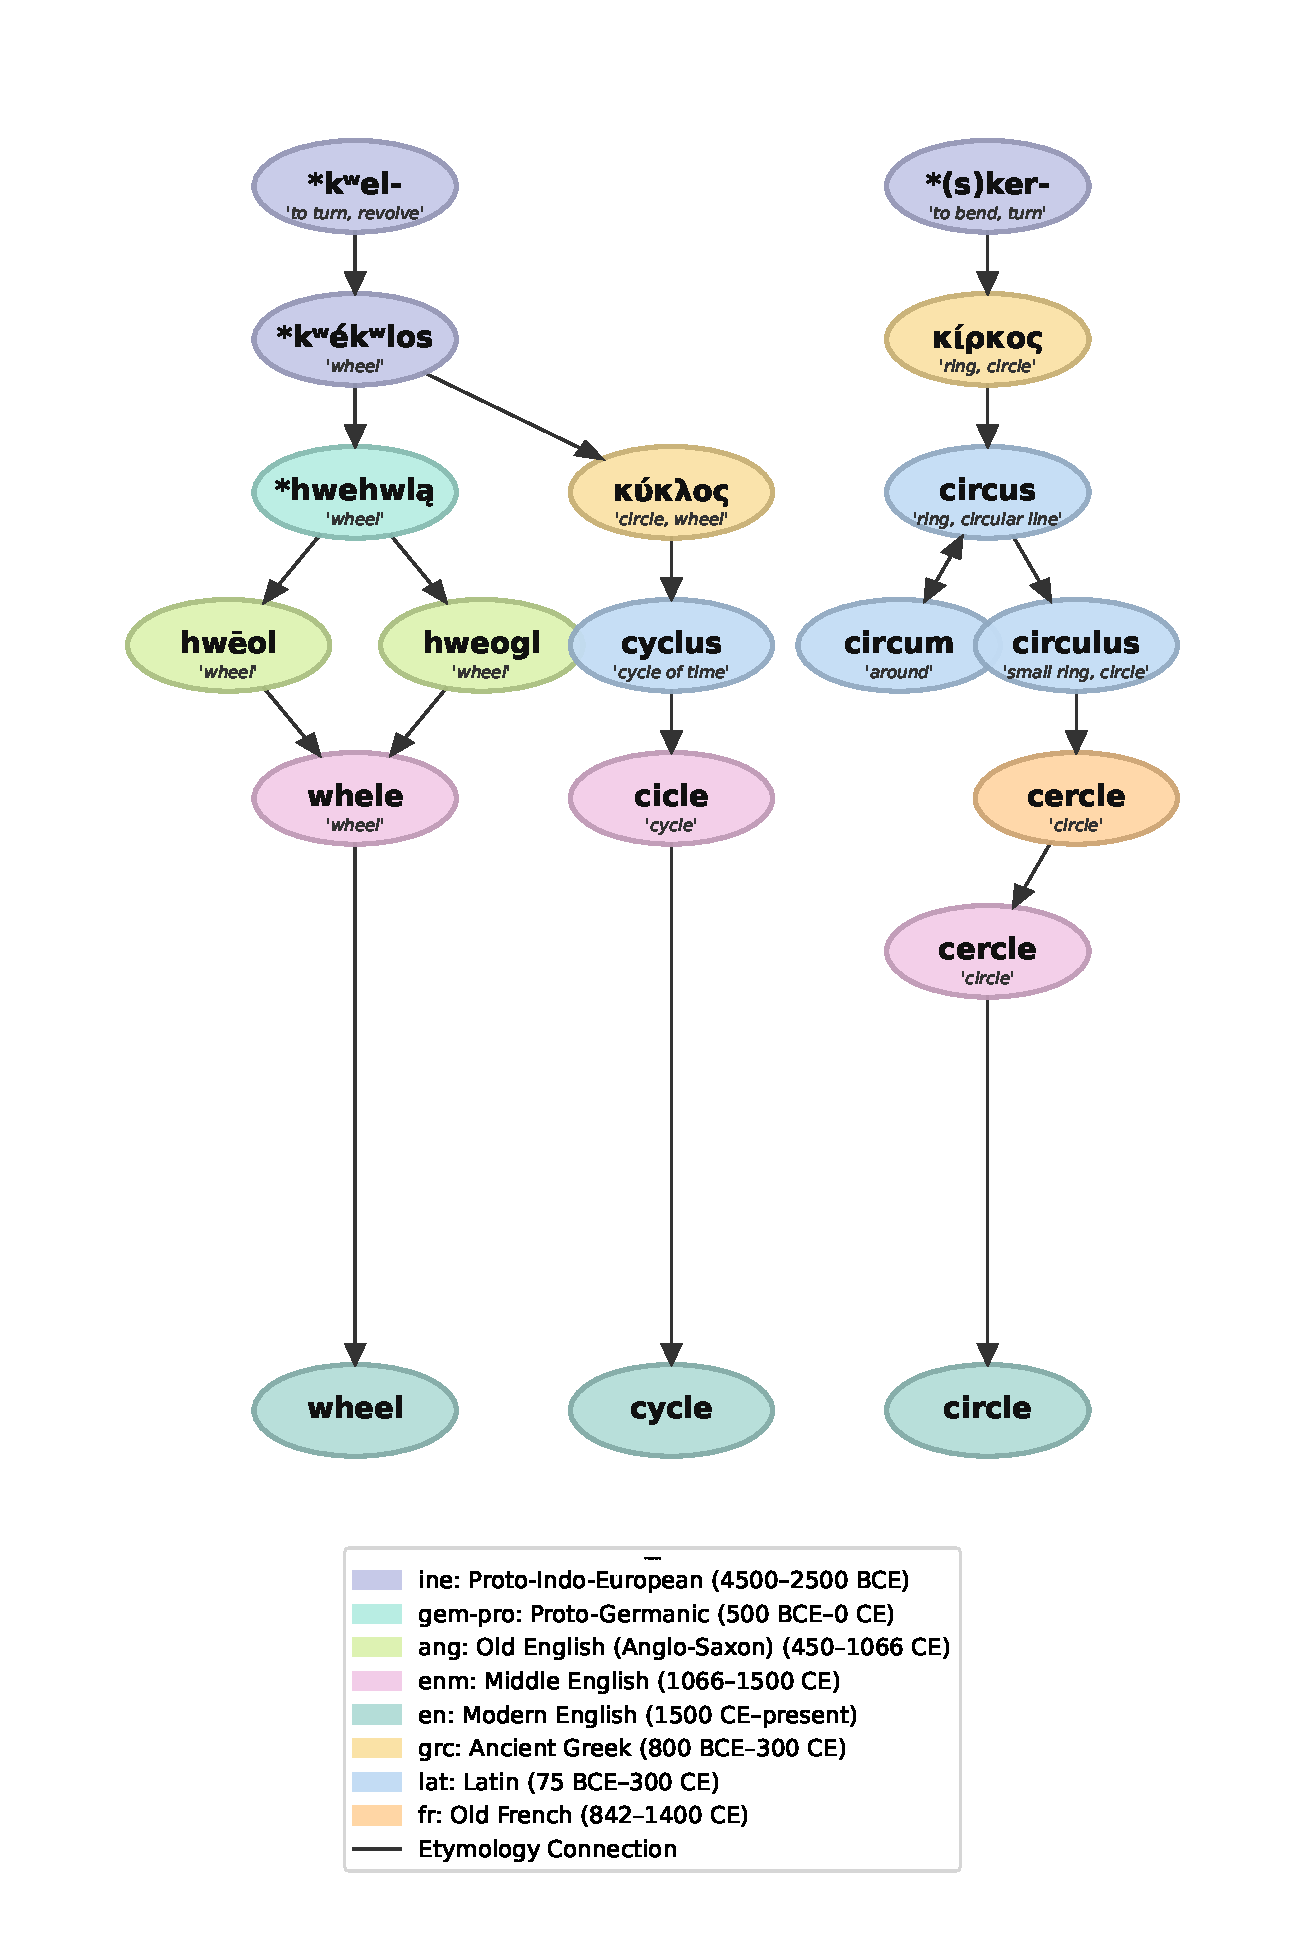
\includegraphics[width=\textwidth,height=\textheight,keepaspectratio]{05_CircleWheel/etymology_graph_portrait_v105.pdf}}
\end{figure}

\begin{SideNotePage}{
  \textbf{Indo-European Language Family Tree:} This phylogenetic reconstruction illustrates the hierarchical relationships among Indo-European languages, flowing from Proto-Indo-European (PIE) on the left to modern languages on the right. The tree demonstrates the systematic branching described by the comparative method, where shared innovations define intermediate nodes and regular sound correspondences link ancestral forms to their descendants.
  
  \vspace{0.5em}
  The diagram directly supports the etymological analysis presented in this chapter. The PIE root \piefont{*kʷékʷlos} ("wheel, circle") appears across multiple branches with predictable phonological transformations: Greek \textgreek{κύκλος} (\emph{kyklos}) via labiovelar to velar shift, Sanskrit \textsanskrit{चक्र} (\emph{chakra}) through labiovelar palatalization, and English "wheel" via Grimm's Law (\piefont{*kʷ} > \piefont{hw}). Each pathway reflects the systematic sound changes that characterize individual language families.
  
  \vspace{0.5em}
  Major branches are color-coded: Germanic (red) encompasses English, German, and Scandinavian languages; Celtic (green) includes Irish and Welsh; Italic (purple) covers Latin and its descendants; Balto-Slavic (blue) spans Russian, Polish, and Baltic languages; Indo-Iranian (orange) includes Hindi, Persian, and related languages. The tree structure reveals how morphological and phonological innovations spread through subgroups while preserving traces of the common ancestral system.
  
  \vspace{0.5em}
  This visualization embodies the principle that historical linguistics can reconstruct unattested languages through structural regularities. The consistency of sound correspondences across the tree — from PIE labiovelars to their various reflexes, from voiced aspirated stops to their systematic outcomes — demonstrates how the comparative method recovers deep linguistic history through systematic analysis of surface-level diversity. The geometric form of the tree reflects the nested structure of shared innovations that define genealogical relationships among related languages.
}{05_CircleWheel/indo_european_tree_tall.pdf}
\end{SideNotePage}